% questions.tex —— 2016 年·江苏卷 · 题目内容片段（无答案）
% 由 tools/generate_projects.py 依来源总账自 2016/2016_数学真题_江苏_试题.md 生成，勿手改（改源 MD 后重跑）


\gkpart{数学}

\begin{gktip}
\textbf{来源说明}：本题面依据固定源 PDF 两页 A3 页面逐题核对，原卷印刷页码 997–998。固定源不附答案、\textbf{不印分值}（全字符集普查：「分」字 6 处皆在词语内部，无「（N 分）」形态）；本文件仅为题面规范源。源内中文标点一律为半角，本文件按项目约定统一为全角；源内异常一律照录并在 \texttt{.work} 版式文件中逐条登记（第 11 题两条大绝对值竖线与第 16 题(1) 的「$\parallel$」在源文本层缺失、系矢量绘制，已照源补出；cases 花括号与矩阵方括号为大定界符分片拼合；向量箭头为 TeX-vect10 绘制；第 6 题流程图的判断支路标签为拉丁 N/Y；第 13 题图中 A/E/F 三处箭头与线段留白、第 16 题图内 F 非 \(B_{1}B\) 中点、第 21 题【A】直角为示意作图，均照源复刻）。

\textbf{结构}：填空题 1–14、解答题 15–20；第 21 题为\textbf{四选二}（下辖【A】–【D】四个选做题，源内于 21 题题号行印「四选二」），21–23 系江苏卷数学Ⅱ附加题段——\textbf{源内 21–23 段前无节标题}（全文无「附加题」「数学Ⅱ」字样），归属判定依据见 \texttt{.work} 登记。
\end{gktip}

\gkpart{一、填空题}

\begin{question}
\gkti{1}已知集合 \(A=\{-1,2,3,6\}\)，\(B=\{x\mid-2<x<3\}\)，则 \(A\cap B=\)\gkblank{}。

\end{question}
\begin{question}
\gkti{2}复数 \(z=(1+2\mathrm{i})(3-\mathrm{i})\)，其中 \(\mathrm{i}\) 为虚数单位，则 \(z\) 的实部是\gkblank{}。

\end{question}
\begin{question}
\gkti{3}在平面直角坐标系 \(xOy\) 中，双曲线 \(\dfrac{x^{2}}{7}-\dfrac{y^{2}}{3}=1\) 的焦距是\gkblank{}。

\end{question}
\begin{question}
\gkti{4}已知一组数据 4.7，4.8，5.1，5.4，5.5，则该组数据的方差是\gkblank{}。

\end{question}
\begin{question}
\gkti{5}函数 \(y=\sqrt{3-2x-x^{2}}\) 的定义域是\gkblank{}。

\Needspace{0.4\textheight}
\end{question}
\begin{question}
\gkti{6}如图是一个算法的流程图，则输出 \(a\) 的值是\gkblank{}。
\nopagebreak[4]
\begin{center}% 第 6 题程序框图（本项目首例流程图类图元）：按固定源 PDF 矢量路径换算（1 pt → 0.03515 cm）。
% 原点取图左下角（源页 (154.98, 500.84) pt），y 向上。
% 结构：自上而下主干 + 右侧回环（b←b−2 在右上、a←a+4 在右中）；判断支路标签为拉丁 N/Y（照源，非「否/是」）。
% 节点：圆角矩形 2（起止框，圆角半径 3.99）、矩形 4、菱形 1（半宽 34.82、半高 8.64）、平行四边形 1（斜移 6.13）。
% 8 条连线（含回环折线）+ 8 个实心箭头（2.99×3.98，尖点在目标端；源内线段在箭头前收笔，照源）。
\begin{tikzpicture}[line cap=round,line join=round,font=\small,x=0.03515cm,y=0.03515cm]
% ===== 连线（8 条）=====
\draw (34.81,171.83)--(34.81,161.25);   % 开始 → a←1
\draw (34.81,143.50)--(34.81,132.92);   % a←1 → b←9
\draw (34.81,114.65)--(34.81,84.23);    % b←9 → 菱形（回接点在上）
\draw (69.91,71.73)--(80.49,71.73);     % 菱形 N 支 → a←a+4
\draw (110.52,79.24)--(110.52,89.82);   % a←a+4 → b←b−2（自下而上）
\draw (85.12,101.19)--(38.40,101.19);   % b←b−2 → 主干（自右向左回接）
\draw (34.81,62.80)--(34.81,52.22);     % 菱形 Y 支 → 输出 a
\draw (34.82,31.38)--(34.81,20.80);     % 输出 a → 结束
% ===== 节点（8 个）=====
\draw[rounded corners=3.99pt] (20.82,172.03)--(48.81,172.03)--(48.81,188.86)--(20.82,188.86)--cycle;  % 开始
\draw (17.75,143.70)--(51.88,143.70)--(51.88,157.46)--(17.75,157.46)--cycle;   % a←1
\draw (18.28,114.85)--(51.35,114.85)--(51.35,129.14)--(18.28,129.14)--cycle;   % b←9
\draw (85.32,93.61)--(135.73,93.61)--(135.73,108.77)--(85.32,108.77)--cycle;   % b←b−2
\draw (69.62,71.73)--(34.81,80.37)--(0,71.73)--(34.81,63.09)--cycle;            % 菱形 a>b
\draw (84.27,64.41)--(136.77,64.41)--(136.77,79.04)--(84.27,79.04)--cycle;     % a←a+4
\draw (10.16,31.58)--(16.29,48.43)--(59.46,48.43)--(53.33,31.58)--cycle;       % 平行四边形 输出 a
\draw[rounded corners=3.99pt] (20.82,0)--(48.81,0)--(48.81,17.01)--(20.82,17.01)--cycle;  % 结束
% ===== 实心箭头（8 个，2.99×3.98）=====
\fill (34.81,157.46)--(33.32,161.44)--(36.30,161.44)--cycle;
\fill (34.81,129.14)--(33.32,133.12)--(36.30,133.12)--cycle;
\fill (34.81,80.37)--(33.32,84.35)--(36.30,84.35)--cycle;
\fill (110.52,93.61)--(109.03,89.63)--(112.01,89.63)--cycle;
\fill (34.81,48.43)--(33.32,52.41)--(36.30,52.41)--cycle;
\fill (34.81,17.01)--(33.32,20.99)--(36.30,20.99)--cycle;
\fill (84.27,71.73)--(80.29,70.24)--(80.29,73.22)--cycle;
\fill (34.81,101.19)--(38.79,99.70)--(38.79,102.68)--cycle;
% ===== 标签（照源字框中心，显式坐标）=====
\node[anchor=center,inner sep=0] at (34.75,180.44) {开始};
\node[anchor=center,inner sep=0] at (34.60,150.64) {\(a\leftarrow 1\)};
\node[anchor=center,inner sep=0] at (35.01,121.87) {\(b\leftarrow 9\)};
\node[anchor=center,inner sep=0] at (110.58,101.56) {\(b\leftarrow b-2\)};
\node[anchor=center,inner sep=0] at (34.95,71.71) {\(a>b\)};
\node[anchor=center,inner sep=0] at (69.90,78.99) {N};
\node[anchor=center,inner sep=0] at (110.37,71.90) {\(a\leftarrow a+4\)};
\node[anchor=center,inner sep=0] at (42.44,55.72) {Y};
\node[anchor=center,inner sep=0] at (34.81,40.01) {输出 \(a\)};
\node[anchor=center,inner sep=0] at (34.83,8.50) {结束};
\end{tikzpicture}
\end{center}
\nopagebreak[4]
\end{question}
\begin{question}
\gkti{7}将一个质地均匀的骰子（一种各个面上分别标有 1，2，3，4，5，6 六个点的正方体玩具）先后抛掷 2 次，则出现向上的点数之和小于 10 的概率是\gkblank{}。

\end{question}
\begin{question}
\gkti{8}已知 \(\{a_{n}\}\) 是等差数列，\(S_{n}\) 是其前 \(n\) 项和。若 \(a_{1}+a_{2}^{2}=-3\)，\(S_{5}=10\)，则 \(a_{9}\) 的值是\gkblank{}。

\end{question}
\begin{question}
\gkti{9}定义在区间 \([0,3\pi]\) 上的函数 \(y=\sin 2x\) 的图象与 \(y=\cos x\) 的图象的交点个数是\gkblank{}。

\Needspace{0.4\textheight}
\end{question}
\begin{question}
\gkti{10}如图，在平面直角坐标系 \(xOy\) 中，\(F\) 是椭圆 \(\dfrac{x^{2}}{a^{2}}+\dfrac{y^{2}}{b^{2}}=1\)（\(a>b>0\)）的右焦点，直线 \(y=\dfrac{b}{2}\) 与椭圆交于 \(B\)，\(C\) 两点，且 \(\angle BFC=90^{\circ}\)，则该椭圆的离心率是\gkblank{}。
\nopagebreak[4]
\begin{center}% 第 10 题椭圆图：按固定源 PDF 矢量路径换算（1 pt → 0.03515 cm）。
% 原点取椭圆中心 O（源页 (220.21, 747.97) pt），y 向上。
% 椭圆半轴 49.08×28.34（b/a=1/√3，源为按题设精确作图），线宽 0.8pt（其余图元 2 倍）；
% x 轴左 −62.33 右至箭头尖点 62.34；y 轴下 −36.83 上至箭头尖点 36.84。
% 弦 y=b/2（过 B、C）、线段 BF/CF、F 处直角记号（三折线）照源；
% O、F 标签在 x 轴下方（源内如此，照录）。
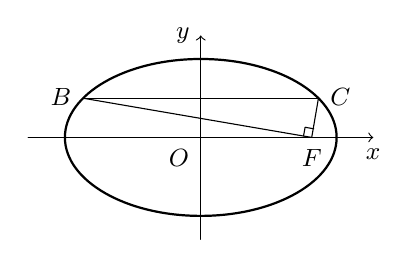
\begin{tikzpicture}[line cap=round,line join=round,font=\small,x=0.03515cm,y=0.03515cm]
% 坐标轴
\draw[->] (-62.33,0)--(62.34,0);
\draw[->] (0,-36.83)--(0,36.84);
% 椭圆（线宽 0.8，与源一致）
\draw[line width=0.8pt] (0,0) ellipse (49.08 and 28.34);
% 弦与焦点弦
\draw (-42.50,14.17)--(42.51,14.17);   % 弦 y=b/2（B–C）
\draw (-42.50,14.17)--(40.08,0);       % B–F
\draw (40.08,0)--(42.51,14.17);        % F–C
\draw (37.13,0.57)--(37.69,3.68)--(40.81,3.12);  % F 处直角记号
% ===== 标注（照源字框中心，显式坐标）=====
\node[anchor=center,inner sep=0] at (-6.49,36.84) {\(y\)};
\node[anchor=center,inner sep=0] at (-50.50,14.73) {\(B\)};
\node[anchor=center,inner sep=0] at (50.47,14.74) {\(C\)};
\node[anchor=center,inner sep=0] at (-7.84,-7.28) {\(O\)};
\node[anchor=center,inner sep=0] at (40.13,-7.30) {\(F\)};
\node[anchor=center,inner sep=0] at (62.26,-5.95) {\(x\)};
\end{tikzpicture}
\end{center}
\nopagebreak[4]
\end{question}
\begin{question}
\gkti{11}设 \(f(x)\) 是定义在 \(\mathbf{R}\) 上且周期为 2 的函数，在区间 \([-1,1)\) 上
\nopagebreak[4]
\[
f(x)=
\begin{cases}
x+a, & -1\leqslant x<0,\\
\left|\dfrac{2}{5}-x\right|, & 0\leqslant x<1,
\end{cases}
\]
其中 \(a\in\mathbf{R}\)。若 \(f\left(-\dfrac{5}{2}\right)=f\left(\dfrac{9}{2}\right)\)，则 \(f(5a)\) 的值是\gkblank{}。

\end{question}
\begin{question}
\gkti{12}已知实数 \(x\)，\(y\) 满足
\nopagebreak[4]
\[
\begin{cases}
x-2y+4\geqslant 0,\\
2x+y-2\geqslant 0,\\
3x-y-3\leqslant 0,
\end{cases}
\]
则 \(x^{2}+y^{2}\) 的取值范围是\gkblank{}。

\Needspace{0.4\textheight}
\end{question}
\begin{question}
\gkti{13}如图，在 \(\triangle ABC\) 中，\(D\) 是 \(BC\) 的中点，\(E\)，\(F\) 是 \(AD\) 上两个三等分点，\(\overrightarrow{BA}\cdot\overrightarrow{CA}=4\)，\(\overrightarrow{BF}\cdot\overrightarrow{CF}=-1\)，则 \(\overrightarrow{BE}\cdot\overrightarrow{CE}\) 的值是\gkblank{}。
\nopagebreak[4]
\begin{center}% 第 13 题平面几何图（三角形 + 三等分点）：按固定源 PDF 矢量路径换算（1 pt → 0.03515 cm）。
% 原点取 B 点（源页 (554.98, 317.76) pt），y 向上。
% A 在上、B 左下、C 右下；D 为 BC 中点，E、F 为 AD 三等分点（E 近 A、F 近 D）。
% 自 B、C 分别向 A、E、F 连线（6 条，均在到达目标点前约 3.6–3.8 pt 处收笔，留白给箭头——照源）；
% 另有底边 BC 与中线 AD；A、E、F 三点处各一个实心箭头（指向该点）。
% 直角等几何按源矢量复刻（源内为示意，非严格作图）。
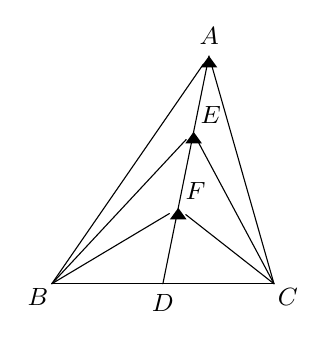
\begin{tikzpicture}[line cap=round,line join=round,font=\small,x=0.03515cm,y=0.03515cm]
% ===== 线段（8 条）=====
\draw (0,0)--(80.26,0);            % B–C（底边）
\draw (0,0)--(54.76,79.35);        % B–A
\draw (80.26,0)--(57.78,78.85);    % C–A
\draw (40.13,0)--(56.79,82.30);    % D–A（中线）
\draw (0,0)--(48.57,52.13);        % B–E
\draw (80.26,0)--(52.70,51.59);    % C–E
\draw (0,0)--(42.48,25.37);        % B–F
\draw (80.26,0)--(48.40,24.99);    % C–F
% ===== 箭头（3 处，各一个实心三角形，指向 A/E/F）=====
\fill (56.79,82.30)--(53.79,78.15)--(59.79,78.15)--cycle;   % → A
\fill (51.24,54.87)--(48.24,50.72)--(54.24,50.72)--cycle;   % → E
\fill (45.68,27.43)--(42.68,23.28)--(48.68,23.28)--cycle;   % → F
% ===== 标注（照源字框中心，显式坐标）=====
\node[anchor=center,inner sep=0] at (56.84,89.44) {\(A\)};
\node[anchor=center,inner sep=0] at (-4.99,-4.93) {\(B\)};
\node[anchor=center,inner sep=0] at (85.33,-4.93) {\(C\)};
\node[anchor=center,inner sep=0] at (40.07,-6.98) {\(D\)};
\node[anchor=center,inner sep=0] at (57.40,61.08) {\(E\)};
\node[anchor=center,inner sep=0] at (51.96,33.53) {\(F\)};
\end{tikzpicture}
\end{center}
\nopagebreak[4]
\end{question}
\begin{question}
\gkti{14}在锐角 \(\triangle ABC\) 中，\(\sin A=2\sin B\sin C\)，则 \(\tan A\tan B\tan C\) 的最小值是\gkblank{}。

\end{question}
\gkpart{二、解答题}

\begin{question}
\gkti{15}在 \(\triangle ABC\) 中，\(AC=6\)，\(\cos B=\dfrac{4}{5}\)，\(C=\dfrac{\pi}{4}\)。

（1） 求 \(AB\) 的长；

（2） 求 \(\cos\left(A-\dfrac{\pi}{6}\right)\) 的值。

\Needspace{0.4\textheight}
\end{question}
\begin{question}
\gkti{16}如图，在直三棱柱 \(ABC-A_{1}B_{1}C_{1}\) 中，\(D\)，\(E\) 分别为 \(AB\)，\(BC\) 的中点，点 \(F\) 在侧棱 \(B_{1}B\) 上，且 \(B_{1}D\perp A_{1}F\)，\(A_{1}C_{1}\perp A_{1}B_{1}\)。求证：

（1） 直线 \(DE\parallel\) 平面 \(A_{1}C_{1}F\)；

（2） 平面 \(B_{1}DE\perp\) 平面 \(A_{1}C_{1}F\)。
\nopagebreak[4]
\begin{center}% 第 16 题直三棱柱图：按固定源 PDF 矢量路径换算（1 pt → 0.03515 cm）。
% 原点取 A 点（源页 (666.91, 770.95) pt），y 向上。
% 上底面 A₁B₁C₁（C₁ 在后）、下底面 ABC（C 在后）；D 为 AB 中点、E 为 BC 中点、F 在棱 B₁B 上。
% 实线 8 段：下底 AB、侧棱 AA₁/BB₁、上底 B₁A₁ 与 A₁C₁/C₁B₁、辅助线 DB₁ 与 AF；
% 虚线 5 段：被遮挡的 CA/CB/CC₁、C₁F、折线 D–E–B₁（V 形，两段均取虚线）。
% 注：源内 F 实测位于自 B₁ 起约 0.446 倍棱长处（非中点；题面仅要求「在 B₁B 上」，照源复刻）。
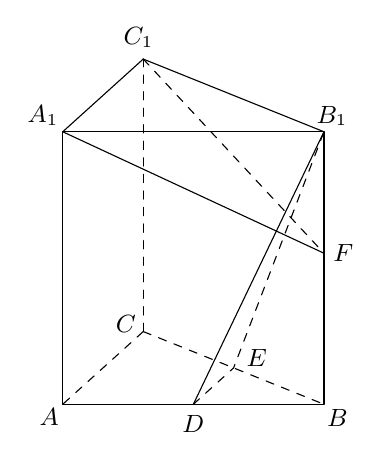
\begin{tikzpicture}[line cap=round,line join=round,font=\small,x=0.03515cm,y=0.03515cm]
% ===== 实线（8 段）=====
\draw (0,0)--(94.36,0);            % A–B
\draw (0,98.44)--(29.08,124.71);   % A₁–C₁
\draw (29.08,124.71)--(94.36,98.44); % C₁–B₁
\draw (94.36,0)--(94.36,98.44);    % B–B₁（过 F）
\draw (94.36,98.44)--(0,98.44);    % B₁–A₁
\draw (0,98.44)--(0,0);            % A₁–A
\draw (47.18,0)--(94.36,98.44);    % D–B₁
\draw (0,98.44)--(94.36,54.57);    % A–F
% ===== 虚线（5 段）=====
\draw[dash pattern=on 2.99pt off 2.99pt] (29.08,26.27)--(94.36,0);    % C–B
\draw[dash pattern=on 2.99pt off 2.99pt] (29.08,26.27)--(0,0);        % C–A
\draw[dash pattern=on 2.99pt off 2.99pt] (29.08,26.27)--(29.08,124.71); % C–C₁
\draw[dash pattern=on 2.99pt off 2.99pt] (29.08,124.71)--(94.36,54.57); % C₁–F
\draw[dash pattern=on 2.99pt off 2.99pt] (47.18,0)--(61.72,13.13)--(94.36,98.44); % D–E–B₁
% ===== 标注（照源字框中心，显式坐标）=====
\node[anchor=center,inner sep=0] at (-7.12,104.33) {\(A_{1}\)};
\node[anchor=center,inner sep=0] at (97.26,104.15) {\(B_{1}\)};
\node[anchor=center,inner sep=0] at (27.35,132.47) {\(C_{1}\)};
\node[anchor=center,inner sep=0] at (-4.88,-4.76) {\(A\)};
\node[anchor=center,inner sep=0] at (99.23,-4.93) {\(B\)};
\node[anchor=center,inner sep=0] at (22.77,28.94) {\(C\)};
\node[anchor=center,inner sep=0] at (47.12,-6.97) {\(D\)};
\node[anchor=center,inner sep=0] at (70.05,16.55) {\(E\)};
\node[anchor=center,inner sep=0] at (101.38,54.56) {\(F\)};
\end{tikzpicture}
\end{center}
\nopagebreak[4]
\Needspace{0.4\textheight}
\end{question}
\begin{question}
\gkti{17}现需要设计一个仓库，它由上下两部分组成，上部分的形状是正四棱锥 \(P-A_{1}B_{1}C_{1}D_{1}\)，下部分的形状是正四棱柱 \(ABCD-A_{1}B_{1}C_{1}D_{1}\)（如图所示），并要求正四棱柱的高 \(O_{1}O\) 是正四棱锥的高 \(PO_{1}\) 的 4 倍。

（1） 若 \(AB=6\ \mathrm{m}\)，\(PO_{1}=2\ \mathrm{m}\)，则仓库的容积是多少？

（2） 若正四棱锥的侧棱长为 \(6\ \mathrm{m}\)，当 \(PO_{1}\) 为多少时，仓库的容积最大？
\nopagebreak[4]
\begin{center}% 第 17 题仓库组合体图（正四棱柱 + 正四棱锥，本项目首例组合体）：按固定源 PDF 矢量路径换算（1 pt → 0.03515 cm）。
% 原点取 A 点（源页 (1033.48, 292.36) pt），y 向上。
% 下部正四棱柱 ABCD-A₁B₁C₁D₁（斜二测，前表面与右表面可见）；
% 上部正四棱锥 P-A₁B₁C₁D₁（叠在顶面上，四条侧棱均实线）。
% 实线 12 段（棱锥 4 侧棱 + 顶面前/右/左 3 棱 + 底面可见棱 + 3 条可见侧棱）；
% 虚线 5 段（被遮挡的 AD/DC/DD₁/C₁D₁ + 竖直中轴虚线 O–O₁–P 一条，串联两高的共线关系）。
% O、O₁ 处实心点（源内标签在左、点在右）；照源复刻。
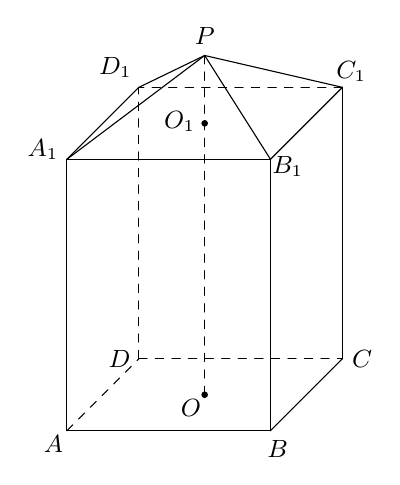
\begin{tikzpicture}[line cap=round,line join=round,font=\small,x=0.03515cm,y=0.03515cm]
% ===== 实线（12 段）=====
\draw (49.76,135.54)--(0,98.04);       % P–A₁
\draw (49.76,135.54)--(73.53,98.04);   % P–B₁
\draw (49.76,135.54)--(99.52,124.03);  % P–C₁
\draw (49.76,135.54)--(25.99,124.03);  % P–D₁
\draw (0,98.04)--(73.53,98.04);        % A₁–B₁（顶面前棱）
\draw (73.53,98.04)--(99.52,124.03);   % B₁–C₁（顶面右棱）
\draw (25.99,124.03)--(0,98.04);       % D₁–A₁（顶面左棱）
\draw (0,0)--(73.53,0);                % A–B（底面前棱）
\draw (73.53,0)--(99.52,25.99);        % B–C（底面右棱）
\draw (0,0)--(0,98.04);                % A–A₁（前左侧棱）
\draw (73.53,0)--(73.53,98.04);        % B–B₁（前右侧棱）
\draw (99.52,25.99)--(99.52,124.03);   % C–C₁（后右侧棱）
% ===== 虚线（5 段）=====
\draw[dash pattern=on 2.99pt off 2.99pt] (0,0)--(25.99,25.99);         % A–D
\draw[dash pattern=on 2.99pt off 2.99pt] (25.99,25.99)--(99.52,25.99); % D–C
\draw[dash pattern=on 2.99pt off 2.99pt] (25.99,25.99)--(25.99,124.03); % D–D₁
\draw[dash pattern=on 2.99pt off 2.99pt] (99.52,124.03)--(25.99,124.03); % C₁–D₁
\draw[dash pattern=on 2.99pt off 2.99pt] (49.76,12.99)--(49.76,135.54); % O–O₁–P（两高共线）
% ===== 实心点（O、O₁ 处）=====
\fill (49.76,12.99) circle (1.2pt);
\fill (49.76,111.03) circle (1.2pt);
% ===== 标注（照源字框中心，显式坐标；O/O₁ 标签在点之左）=====
\node[anchor=center,inner sep=0] at (49.83,142.51) {\(P\)};
\node[anchor=center,inner sep=0] at (17.51,131.15) {\(D_{1}\)};
\node[anchor=center,inner sep=0] at (102.73,129.75) {\(C_{1}\)};
\node[anchor=center,inner sep=0] at (-8.63,101.66) {\(A_{1}\)};
\node[anchor=center,inner sep=0] at (79.78,95.39) {\(B_{1}\)};
\node[anchor=center,inner sep=0] at (18.96,25.98) {\(D\)};
\node[anchor=center,inner sep=0] at (106.63,25.99) {\(C\)};
\node[anchor=center,inner sep=0] at (-4.89,-4.76) {\(A\)};
\node[anchor=center,inner sep=0] at (76.14,-6.45) {\(B\)};
\node[anchor=center,inner sep=0] at (40.70,111.82) {\(O_{1}\)};
\node[anchor=center,inner sep=0] at (44.83,8.06) {\(O\)};
\end{tikzpicture}
\end{center}
\nopagebreak[4]
\Needspace{0.4\textheight}
\end{question}
\begin{question}
\gkti{18}如图，在平面直角坐标系 \(xOy\) 中，已知以 \(M\) 为圆心的圆 \(M\)：\(x^{2}+y^{2}-12x-14y+60=0\) 及其上一点 \(A(2,4)\)。

（1） 设圆 \(N\) 与 \(x\) 轴相切，与圆 \(M\) 外切，且圆心 \(N\) 在直线 \(x=6\) 上，求圆 \(N\) 的标准方程；

（2） 设平行于 \(OA\) 的直线 \(l\) 与圆 \(M\) 相交于 \(B\)，\(C\) 两点，且 \(BC=OA\)，求直线 \(l\) 的方程；

（3） 设点 \(T(t,0)\) 满足：存在圆 \(M\) 上的两点 \(P\) 和 \(Q\)，使得 \(\overrightarrow{TA}+\overrightarrow{TP}=\overrightarrow{TQ}\)，求实数 \(t\) 的取值范围。
\nopagebreak[4]
\begin{center}% 第 18 题圆 M 坐标图：按固定源 PDF 矢量路径换算（1 pt → 0.03515 cm）。
% 原点取 O（源页 (1030.25, 675.27) pt），y 向上。
% 圆线宽 0.8pt（其余图元 2 倍）；圆心 M (55.43,64.66)、半径 46.19；
% 圆上定点 A（题设 A(2,4) 的精确作图位置，正比 9.238 pt/单位）；M、A 处实心点。
% x 轴左 −18.48 右至箭头尖点 110.85；y 轴下 −18.48 上至箭头尖点 120.09。
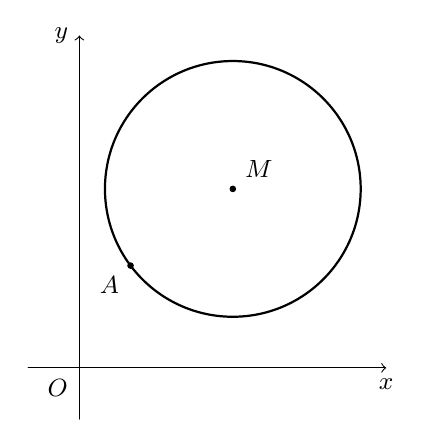
\begin{tikzpicture}[line cap=round,line join=round,font=\small,x=0.03515cm,y=0.03515cm]
% 坐标轴
\draw[->] (-18.48,0)--(110.85,0);
\draw[->] (0,-18.48)--(0,120.09);
% 圆（线宽 0.8，与源一致）
\draw[line width=0.8pt] (55.43,64.66) circle (46.19);
% 实心点（M、A）
\fill (55.43,64.66) circle (1.2pt);
\fill (18.48,36.95) circle (1.2pt);
% ===== 标注（照源字框中心，显式坐标）=====
\node[anchor=center,inner sep=0] at (-6.50,120.09) {\(y\)};
\node[anchor=center,inner sep=0] at (64.83,71.94) {\(M\)};
\node[anchor=center,inner sep=0] at (10.88,29.84) {\(A\)};
\node[anchor=center,inner sep=0] at (-7.85,-7.29) {\(O\)};
\node[anchor=center,inner sep=0] at (110.77,-5.96) {\(x\)};
\end{tikzpicture}
\end{center}
\nopagebreak[4]
\end{question}
\begin{question}
\gkti{19}已知函数 \(f(x)=a^{x}+b^{x}\)（\(a>0\)，\(b>0\)，\(a\neq1\)，\(b\neq1\)）。

（1） 设 \(a=2\)，\(b=\dfrac{1}{2}\)。

① 求方程 \(f(x)=2\) 的根；

② 若对于任意 \(x\in\mathbf{R}\)，不等式 \(f(2x)\geqslant mf(x)-6\) 恒成立，求实数 \(m\) 的最大值；

（2） 若 \(0<a<1\)，\(b>1\)，函数 \(g(x)=f(x)-2\) 有且只有 1 个零点，求 \(ab\) 的值。

\end{question}
\begin{question}
\gkti{20}记 \(U=\{1,2,\cdots,100\}\)。对数列 \(\{a_{n}\}\)（\(n\in\mathbf{N}^{*}\)）和 \(U\) 的子集 \(T\)，若 \(T=\varnothing\)，定义 \(S_{T}=0\)；若 \(T=\{t_{1},t_{2},\cdots,t_{k}\}\)，定义 \(S_{T}=a_{t_{1}}+a_{t_{2}}+\cdots+a_{t_{k}}\)。例如：\(T=\{1,3,66\}\) 时，\(S_{T}=a_{1}+a_{3}+a_{66}\)。现设 \(\{a_{n}\}\)（\(n\in\mathbf{N}^{*}\)）是公比为 3 的等比数列，且当 \(T=\{2,4\}\) 时，\(S_{T}=30\)。

（1） 求 \(\{a_{n}\}\) 的通项公式；

（2） 对任意正整数 \(k\)（\(1\leqslant k\leqslant 100\)），若 \(T\subseteq\{1,2,\cdots,k\}\)，求证：\(S_{T}<a_{k+1}\)；

（3） 设 \(C\subseteq U\)，\(D\subseteq U\)，\(S_{C}\geqslant S_{D}\)，求证：\(S_{C}+S_{C\cap D}\geqslant 2S_{D}\)。

\Needspace{0.4\textheight}
\end{question}
\begin{question}
\gkti{21}四选二。

【A】如图，在 \(\triangle ABC\) 中，\(\angle ABC=90^{\circ}\)，\(BD\perp AC\)，\(D\) 为垂足，\(E\) 是 \(BC\) 中点。求证：\(\angle EDC=\angle ABD\)。
\nopagebreak[4]
\begin{center}% 第 21 题【A】直角三角形图：按固定源 PDF 矢量路径换算（1 pt → 0.03515 cm）。
% 原点取 A 点（源页 (653.07, 180.07) pt），y 向上。
% A 左下、C 右下（AC 水平为斜边）、B 上方（直角顶点，∠ABC=90° 由题面保证）；
% D 为 B 到 AC 的垂足；E 为 BC 中点，连 DE。
% 注：源图为示意性（BA 与 BC 斜率积 ≈ −0.946，非严格垂直；图中未画直角记号），照源复刻。
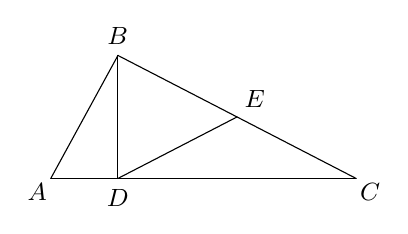
\begin{tikzpicture}[line cap=round,line join=round,font=\small,x=0.03515cm,y=0.03515cm]
\draw (0,0)--(24.26,44.43);      % A–B（直角边）
\draw (0,0)--(110.29,0);         % A–C（斜边，过 D）
\draw (24.26,44.43)--(24.26,0);  % B–D（斜边上的高）
\draw (24.26,0)--(67.28,22.21);  % D–E
\draw (24.26,44.43)--(110.29,0); % B–C（另一直角边，过 E）
% ===== 标注（照源字框中心，显式坐标）=====
\node[anchor=center,inner sep=0] at (-4.88,-4.76) {\(A\)};
\node[anchor=center,inner sep=0] at (24.21,51.39) {\(B\)};
\node[anchor=center,inner sep=0] at (115.36,-4.93) {\(C\)};
\node[anchor=center,inner sep=0] at (24.20,-6.98) {\(D\)};
\node[anchor=center,inner sep=0] at (73.66,28.53) {\(E\)};
\end{tikzpicture}
\end{center}
\nopagebreak[4]
【B】已知矩阵 $A=\begin{bmatrix}1&2\\0&-2\end{bmatrix}$，矩阵 \(B\) 的逆矩阵 $B^{-1}=\begin{bmatrix}1&-\dfrac{1}{2}\\0&2\end{bmatrix}$，求矩阵 \(AB\)。

\Needspace{5\baselineskip}
【C】在平面直角坐标系 \(xOy\) 中，已知直线 \(l\) 的参数方程为
\nopagebreak[4]
\[
\begin{cases}
x=1+\dfrac{1}{2}t,\\
y=\dfrac{\sqrt{3}}{2}t,
\end{cases}
\]
\Needspace{5\baselineskip}
（\(t\) 为参数），椭圆 \(C\) 的参数方程为
\nopagebreak[4]
\[
\begin{cases}
x=\cos\theta,\\
y=2\sin\theta,
\end{cases}
\]
（\(\theta\) 为参数）。设直线 \(l\) 与椭圆 \(C\) 相交于 \(A\)，\(B\) 两点，求线段 \(AB\) 的长。

【D】设 \(a>0\)，\(|x-1|<\dfrac{a}{3}\)，\(|y-2|<\dfrac{a}{3}\)，求证：\(|2x+y-4|<a\)。

\Needspace{0.4\textheight}
\end{question}
\begin{question}
\gkti{22}如图，在平面直角坐标系 \(xOy\) 中，已知直线 \(l\)：\(x-y-2=0\)，抛物线 \(C\)：\(y^{2}=2px\)（\(p>0\)）。

（1） 若直线 \(l\) 过抛物线 \(C\) 的焦点，求抛物线 \(C\) 的方程；

（2） 已知抛物线 \(C\) 上存在关于直线 \(l\) 对称的相异两点 \(P\) 和 \(Q\)。

① 求证：线段 \(PQ\) 上的中点坐标为 \((2-p,-p)\)；

② 求 \(p\) 的取值范围。
\nopagebreak[4]
\begin{center}% 第 22 题抛物线图：按固定源 PDF 矢量路径换算（1 pt → 0.03515 cm）。
% 原点取 O（抛物线顶点，源页 (1027.76, 234.91) pt），y 向上。
% 抛物线线宽 0.8pt（其余图元 2 倍），按源精确作图：单位长 14.168 pt、p=1 单位（y²=2px 逐点残差 ≤0.001）；
% 上下两支在 u=6.35 单位（x=89.96）处齐头收笔；直线 l 斜率页面 −1（数学 +1）、截距 ±2 单位，均照源。
% x 轴左 −28.34 右至箭头尖点 113.34；y 轴下 −70.84 上至箭头尖点 70.84；曲线名 C 标注在上支端头旁。
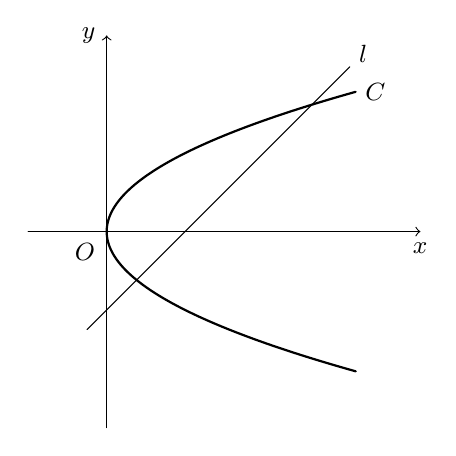
\begin{tikzpicture}[line cap=round,line join=round,font=\small,x=0.03515cm,y=0.03515cm]
% 坐标轴
\draw[->] (-28.34,0)--(113.34,0);
\draw[->] (0,-70.84)--(0,70.84);
% 抛物线（线宽 0.8，与源一致；单位长 14.168）
\draw[line width=0.8pt] plot[domain=-3.5636:3.5636,samples=121] ({(\x*\x/2)*14.168},{\x*14.168});
% 直线 l
\draw (-7.09,-35.42)--(87.84,59.50);
% ===== 标注（照源字框中心，显式坐标）=====
\node[anchor=center,inner sep=0] at (-6.50,70.84) {\(y\)};
\node[anchor=center,inner sep=0] at (92.69,64.37) {\(l\)};
\node[anchor=center,inner sep=0] at (97.08,50.49) {\(C\)};
\node[anchor=center,inner sep=0] at (-7.85,-7.28) {\(O\)};
\node[anchor=center,inner sep=0] at (113.26,-5.96) {\(x\)};
\end{tikzpicture}
\end{center}
\nopagebreak[4]
\end{question}
\begin{question}
\gkti{23}（1） 求 \(7\mathrm{C}_6^3-4\mathrm{C}_7^4\) 的值；

（2） 设 \(m\)，\(n\in\mathbf{N}^{*}\)，\(n\geqslant m\)，求证：\((m+1)\mathrm{C}_m^m+(m+2)\mathrm{C}_{m+1}^m+(m+3)\mathrm{C}_{m+2}^m+\cdots+n\mathrm{C}_{n-1}^m+(n+1)\mathrm{C}_n^m=(m+1)\mathrm{C}_{n+2}^{m+2}\)。

\end{question}